% Original book diagram: fig:bayes-prediction-illustration
% Book source: sections/Part_I/bayesian_prediction.tex
% Original diagram authorship retained. Visual design: Ziad Mosalam.
\documentclass[11pt,border=8pt]{standalone}
\usepackage{amsmath,amssymb,graphicx,tikz}
\usetikzlibrary{arrows.meta,automata,positioning,calc,shapes.geometric,fit,backgrounds,patterns}
\newcommand{\vect}[1]{\mathbf{#1}}
\newcommand{\mat}[1]{\mathbf{#1}}
\newcommand{\Normal}{\mathcal{N}}
\newcommand{\prob}{p}
\newcommand{\E}{\mathbb{E}}
\newcommand{\Var}{\mathrm{Var}}
\newcommand{\Cov}{\mathrm{Cov}}
\newcommand{\CovP}{\mathbf{P}}
\newcommand{\Prob}{\mathbb{P}}
\setlength{\textwidth}{6.5in}
% Shared visual vocabulary for the book's original diagrams.
% Figures opt in explicitly, so unrelated text and existing additions are unchanged.
\definecolor{BookBlue}{HTML}{003262}
\definecolor{BookGold}{HTML}{B17A00}
\definecolor{BookTeal}{HTML}{247C86}
\definecolor{BookInk}{HTML}{30363B}
\definecolor{BookLight}{HTML}{E9EFF5}
\tikzset{
  book figure/.style={font=\small\rmfamily, color=BookBlue, text=BookInk,
    line width=0.8pt, >=Latex},
  book axis/.style={->, draw=BookInk, line width=0.6pt},
  book link/.style={->, draw=BookBlue, line width=0.8pt},
  book observation/.style={draw=BookGold, fill=BookGold!8},
  book state/.style={draw=BookBlue, fill=BookLight},
  book note/.style={font=\footnotesize\rmfamily, text=BookInk}
}

\begin{document}
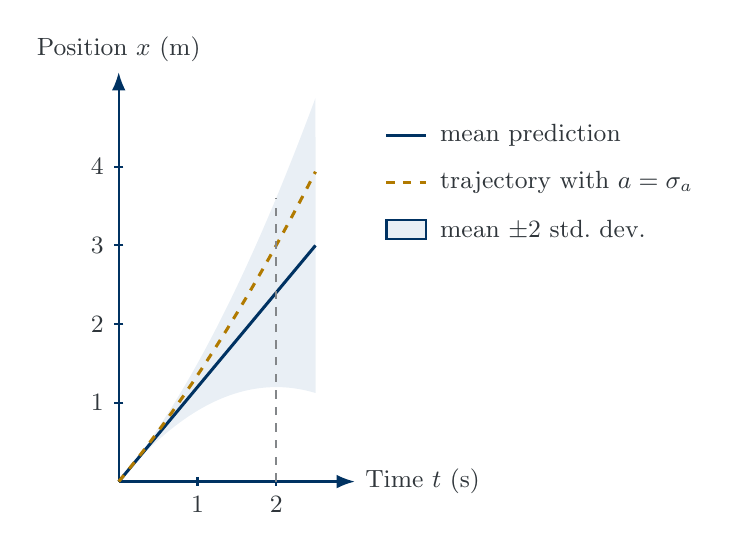
\begin{tikzpicture}[font=\small, text=BookInk, draw=BookBlue, line width=0.8pt, >=Latex, scale=1.0]
% Calibrated to the example: mean 1.2t, standard deviation 0.15t^2 (sigma_a = 0.3 m/s^2)
% shaded band: mean +/- 2 standard deviations
\fill[BookLight, domain=0:2.5, samples=60]
plot (\x, {1.2*\x + 0.3*\x*\x})
-- plot[domain=2.5:0] (\x, {1.2*\x - 0.3*\x*\x})
-- cycle;

% axes and ticks
\draw[->] (0,0) -- (3.0,0) node[right] {Time $t$ (s)};
\draw[->] (0,0) -- (0,5.2) node[above] {Position $x$ (m)};
\foreach \t in {1,2} \draw (\t,0.06) -- (\t,-0.06) node[below] {\small $\t$};
\foreach \y in {1,2,3,4} \draw (0.06,\y) -- (-0.06,\y) node[left] {\small $\y$};

% mean trajectory
\draw[BookBlue, line width=1.1pt, domain=0:2.5, samples=60]
plot (\x, {1.2*\x});

% one possible trajectory (constant acceleration a = +sigma_a)
\draw[BookGold, dashed, line width=1.1pt, domain=0:2.5, samples=60]
plot (\x, {1.2*\x + 0.15*\x*\x});

% prediction horizon
\draw[dashed, BookInk!60] (2,0) -- (2,3.6);

% legend
\begin{scope}[shift={(3.4,3.2)}]
\draw[BookBlue, line width=1.1pt] (0,1.2) -- (0.5,1.2); \node[right] at (0.55,1.2) {\small mean prediction};
\draw[BookGold, dashed, line width=1.1pt] (0,0.6) -- (0.5,0.6); \node[right] at (0.55,0.6) {\small trajectory with $a=\sigma_a$};
\fill[BookLight] (0,-0.12) rectangle (0.5,0.12); \draw (0,-0.12) rectangle (0.5,0.12); \node[right] at (0.55,0) {\small mean $\pm 2$ std.\ dev.};
\end{scope}
\end{tikzpicture}
\end{document}
